%% ============================================================================
%% SafeStream-Redactor: Provably-Equivalent Constant-Memory Streaming Redaction
%% of PII and Credentials
%%
%% Prepared for FTNCT'09 -- Track 4: Cybersecurity, Privacy, and Trust.
%% FTNCT proceedings are published by Springer in the Communications in
%% Computer and Information Science (CCIS) series, which uses the official
%% Springer LNCS author template (llncs.cls), single-column A4, numbered
%% references. This source targets that class.
%% ============================================================================
\documentclass[runningheads]{llncs}

\usepackage[T1]{fontenc}
\usepackage[utf8]{inputenc}
\usepackage{graphicx}
\usepackage{amsmath}
\usepackage{amssymb}
\usepackage{booktabs}
\usepackage{array}
\usepackage{multirow}
\usepackage{makecell}
\usepackage{xcolor}
\usepackage{tikz}
\usetikzlibrary{arrows.meta,positioning,calc,fit,backgrounds}
\usepackage{listings}
\usepackage{algorithm}
\usepackage{algpseudocode}
\usepackage{url}
\usepackage[protrusion=true,expansion=false]{microtype}
% hyperref is loaded last, as recommended; llncs is compatible with it.
\usepackage[hidelinks]{hyperref}

% A compact monospace style for the few inline code fragments.
\lstset{basicstyle=\ttfamily\small,breaklines=true,columns=fullflexible}

% Absorb the few sub-line overfull boxes from long proper nouns / URLs without
% introducing loose interword spacing.
\emergencystretch=1.2em

% Shorthands for the formal objects used throughout.
\newcommand{\T}{T}
\newcommand{\Pipe}{\Pi}
\newcommand{\Sw}{S_{w}}
\newcommand{\Pwk}{P_{w,k}}
\newcommand{\Lmax}{L_{\max}}
\newcommand{\Cleft}{C_{\mathrm{left}}}
\newcommand{\Cright}{C_{\mathrm{right}}}

\begin{document}

\title{SafeStream-Redactor: Provably-Equivalent Constant-Memory Streaming
Redaction of PII and Credentials}

% Per the LNCS template, a short running title is supplied for page headers.
\titlerunning{Provably-Equivalent Streaming Redaction of PII and Credentials}

% Author block left to be completed by the submitting author(s) at
% camera-ready time. Placeholders follow the LNCS template structure.
\author{Anonymous Author(s)}
\authorrunning{Anonymous Author(s)}
\institute{Affiliation withheld for review\\
\email{corresponding.author@example.org}}

\maketitle

% ---------------------------------------------------------------------------
\begin{abstract}
Redacting personally identifiable information (PII) and leaked credentials from
very large text artefacts---logs, database dumps, and exports---forces an
uncomfortable choice: load the whole document into memory (which does not scale)
or process it in chunks (which risks cutting an entity in half at a chunk
boundary). We present \emph{SafeStream-Redactor}, a local-first redaction engine
that resolves this tension with a \emph{bounded-overlap} streaming architecture
whose peak working memory is independent of input size, and we give a
\emph{formal equivalence guarantee}: under two explicitly stated locality
assumptions---bounded span length and bounded context---the streamed output is
identical to an idealised whole-document pass, and the multi-core output is
byte-identical to the sequential pass or the engine transparently falls back to
it through a seam cross-check. The guarantee is stated only for detectors that
satisfy a bounded-window, chunk-independent contract, and the constants
($\Cleft=96$, $\Cright=8$, $\Lmax=8192$) are derived mechanically from the
shipped detectors rather than assumed, and pinned by a regression test. The detection layer is a calibrated ensemble of a deterministic
regex-plus-validator tier, a Shannon-entropy tier for undocumented secrets, a
contextual-scoring tier, and an optional named-entity tier, with a
dependency-free logistic calibrator that turns hand-set confidences into
probabilities. On a self-generated adversarial corpus dense with hard
negatives, the deterministic tier holds precision $0.999$ (45 benign false
positives across 70{,}169 gold spans) with zero missed structured-PII entities;
peak memory stays flat ($2.75$\,MB) as input grows $4\times$, and a 1\,GB file
redacts under a 16\,MB allocation cap. We are explicit about scope: these
corpora are synthetic regression fixtures that measure format coverage and
false-positive resistance, \emph{not} real-world recall, and free-text recall is
a precision/recall trade-off we characterise rather than claim to solve.
\keywords{PII redaction \and secret detection \and streaming algorithms \and
constant memory \and formal equivalence \and data privacy \and named-entity
recognition \and confidence calibration.}
\end{abstract}

% ===========================================================================
\section{Introduction and Contributions}
\label{sec:intro}

Data-protection regulation (e.g.\ the EU General Data Protection
Regulation~\cite{gdpr}) and routine security hygiene both demand that sensitive
values be removed from text before it is shared, archived, or fed to downstream
tooling. Two classes of sensitive value matter in practice: \emph{PII}
(emails, phone numbers, payment-card numbers, national identifiers, IP
addresses, and free-form names and locations) and \emph{credentials/secrets}
(API keys, cloud access keys, service tokens, JWTs, private-key blocks, and
bespoke high-entropy secrets). General-purpose PII engines such as Microsoft
Presidio~\cite{presidio} and scrubadub target the former; dedicated secret
scanners such as gitleaks~\cite{gitleaks} target the latter. Few tools cover
both in a single pass, and---more importantly for this paper---none that we are
aware of \emph{states}, let alone \emph{proves}, that its chunked or parallel
execution produces the same output as processing the whole document at once.

That gap matters because the artefacts most in need of redaction are exactly the
ones too large to hold in memory: multi-gigabyte application logs, incident
captures, and data exports. A naive chunked redactor can silently miss an entity
that straddles a chunk boundary, or emit different output depending on where the
chunks happen to fall---a correctness defect that is invisible until it leaks.

\paragraph{Contributions.}
This paper makes the following contributions, each traceable to the
SafeStream-Redactor implementation that is its sole source of truth:

\begin{enumerate}
\item \textbf{Constant-memory streaming redaction} of PII and credentials in one
pass, with peak working memory bounded by
$\mathit{chunk\_size} + w + \Lmax$ and independent of input size
(Sections~\ref{sec:arch}--\ref{sec:algo}; Theorem~\ref{thm:mem}).
\item \textbf{A bounded-overlap streaming architecture} that carries a rolling
context window between chunks and retreats the emit boundary out of any
straddling detection, so every entity up to the overlap length is seen whole at
least once (Section~\ref{sec:algo}).
\item \textbf{A formal equivalence guarantee} (Section~\ref{sec:formal}) that the
streamed output equals a whole-document reference pass under two explicitly
stated assumptions---\emph{bounded span length} (A1) and \emph{bounded context
locality} (A2)---whose constants are audited from the code. The theorem applies
\emph{only} to detectors satisfying a bounded-window, chunk-independent
contract; we do \emph{not} claim unconditional equivalence for arbitrary
detectors.
\item \textbf{Safe multi-core execution}: a character-aligned range split with a
seam cross-check that yields byte-identical output to the sequential pass, or
transparently falls back to it on seam disagreement---making the parallel path
equal to the sequential path \emph{unconditionally} (Theorem~\ref{thm:par}).
\item \textbf{A calibrated detection ensemble} with a dependency-free logistic
calibrator over detection-local features, and two named operating points---a
precision-favouring \textsc{strict} policy and a recall-favouring
\textsc{high\_recall} policy---exposed through a single confidence threshold
(Section~\ref{sec:semantic}). We present the result as a precision/recall and
benign-false-positive trade-off, not as a solution to free-text recall.
\end{enumerate}

The novelty is not the engineering mechanisms (overlap windows, anchor
prefilters, a seam protocol) individually, but the \emph{guarantee} those
mechanisms admit: a bounded-memory, parallel redactor whose output provably
matches an idealised whole-document pass, with the one failure mode named and
made safe.

% ===========================================================================
\section{Related Work}
\label{sec:related}

\paragraph{PII detection and de-identification.}
Microsoft Presidio~\cite{presidio} is a widely used open-source framework that
combines pattern recognizers with a spaCy/transformer NLP pipeline for entity
recognition. scrubadub offers a simpler rule- and model-based pipeline. In the
clinical domain, Philter~\cite{philter} performs rule-based de-identification of
protected health information, and shared tasks such as the 2014 i2b2/UTHealth
de-identification challenge~\cite{n2c2} established the gold-standard evaluation
methodology for longitudinal clinical narratives. Learned sequence labellers
dominate free-text PII and named-entity recognition: the CoNLL-2003 shared
task~\cite{conll2003} remains a standard NER benchmark, transformer encoders
such as BERT~\cite{bert} set the modern baseline, and recent generalist models
such as GLiNER~\cite{gliner} recognise arbitrary entity types from a prompt.
Surveys of deep-learning NER~\cite{nersurvey} catalogue the precision/recall
trade-offs inherent to free-text entity extraction. SafeStream is regex- and
entropy-first by design, with named-entity recognition as an optional tier; it
therefore trades lower free-text recall for zero required dependencies, local
execution, and the equivalence guarantee below.

\paragraph{Secret and credential detection.}
Secret scanning is a distinct line of work. Meli et al.~\cite{howbadgit}
characterised the prevalence of leaked secrets in public GitHub repositories,
and curated corpora such as SecretBench~\cite{secretbench} now support
systematic evaluation. Tools such as gitleaks~\cite{gitleaks} and entropy-based
heuristics---grounded in Shannon's measure of information~\cite{shannon}---detect
both known-format keys and bespoke high-entropy secrets. General PII engines
typically ship no credential recognizers at all; SafeStream covers both PII and
secrets in the same streaming pass.

\paragraph{Streaming and parallel text processing.}
Constant-memory processing of unbounded input is the central concern of the
data-stream model~\cite{muthukrishnan}. Practical scanning performance depends on
the matching engine: Thompson's NFA construction~\cite{thompson} and the RE2
line of work~\cite{re2} give linear-time regular-expression matching, though, as
we report, lookaround-free and Unicode-boundary-consistent patterns are a
prerequisite for adopting such engines without changing output. What is largely
absent from prior redaction tools is an explicit statement that streaming or
parallel execution is equivalent to a whole-document pass; SafeStream's bounded
overlap and seam protocol are designed precisely to admit such a proof.

\paragraph{Transformation and pseudonymisation.}
Beyond deletion, redactors may mask or pseudonymise values. Keyed deterministic
pseudonymisation (here built on HMAC~\cite{hmac}) preserves referential
integrity across a corpus but, because equal inputs map to equal tokens, it
leaks value equality and is not anonymisation in the sense
of $k$-anonymity~\cite{kanonymity}; we treat it accordingly
(Section~\ref{sec:arch}).

% ===========================================================================
\section{Problem Definition and Design Goals}
\label{sec:problem}

\paragraph{Problem.}
Given an input text $\T$ over a Unicode character alphabet, possibly far larger
than available memory, produce a redacted text in which every detected sensitive
span is rewritten by a redaction policy, while (i) using memory independent of
$|\T|$ and (ii) producing the \emph{same} output a whole-document pass would
produce.

\paragraph{Design goals.}
\begin{description}
\item[G1 -- Constant memory.] Peak working memory must not grow with $|\T|$, so a
100\,GB file redacts in the same footprint class as a 1\,KB one.
\item[G2 -- Boundary correctness.] No entity may be missed or mis-scored merely
because a chunk boundary falls inside it or inside the context it needs.
\item[G3 -- Equivalence under parallelism.] Splitting one file across cores must
yield byte-identical output to the sequential pass, or fail safely to it.
\item[G4 -- Dual coverage.] PII \emph{and} credentials/secrets must be detected
in a single pass.
\item[G5 -- Local-first.] Processing must run fully offline with no required
third-party runtime dependency in the core, so sensitive text never has to leave
the machine.
\item[G6 -- Honest, calibrated confidence.] Detection confidences should be
interpretable as probabilities and expose a principled precision/recall knob,
rather than an arbitrary threshold.
\end{description}

\paragraph{Non-goals.}
We do not target the widest possible catalogue of built-in entity types, managed
cloud scale, multilingual coverage, or enterprise data-governance workflows;
these are better served by cloud DLP and governance platforms. We also do not
claim to solve free-text recall: names, street addresses, and format-less
identifiers have no distinctive shape, and any detector faces an irreducible
precision/recall trade-off on them.

% ===========================================================================
\section{SafeStream-Redactor Architecture}
\label{sec:arch}

Figure~\ref{fig:arch} shows the layered architecture. A coordination layer
(\texttt{Redactor}) drives the streaming engine, which feeds text windows to a
cascade of detection tiers whose outputs are scored, filtered, and
overlap-resolved before a redaction policy rewrites the text.

\begin{figure}[t]
\centering
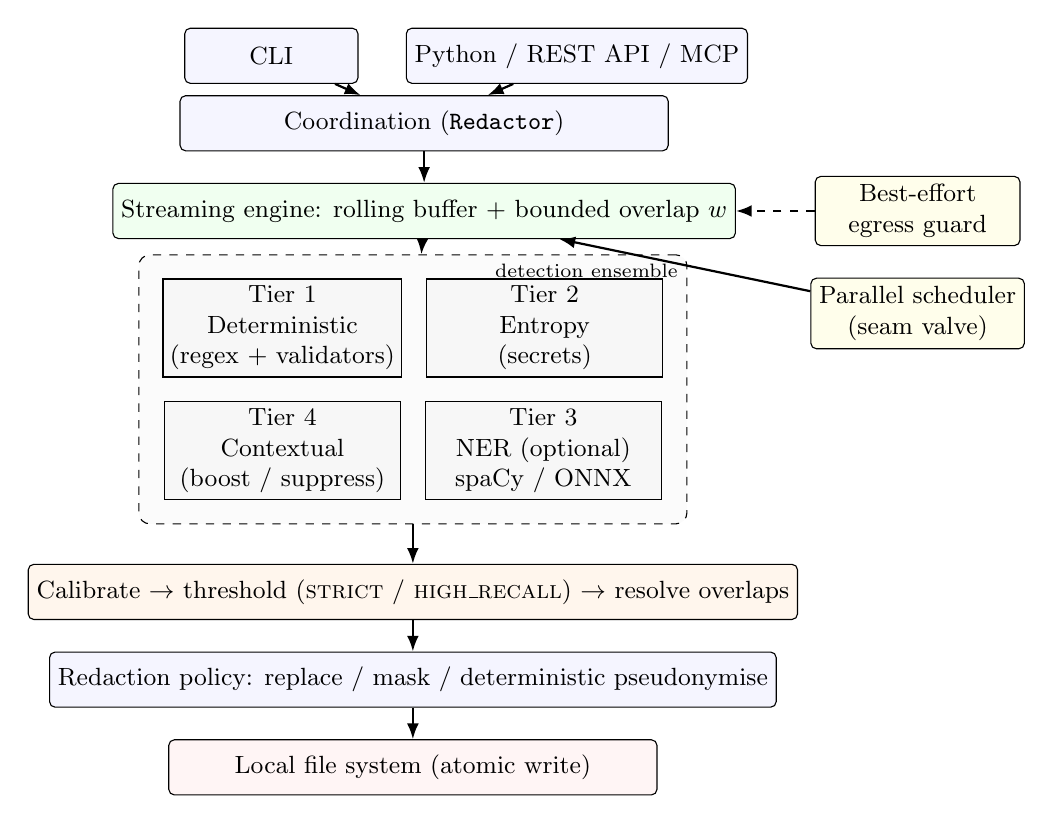
\begin{tikzpicture}[
  font=\small,
  box/.style={draw,rounded corners=2pt,align=center,minimum height=7mm,
    inner sep=3pt,fill=blue!4},
  tier/.style={draw,align=center,minimum height=6.5mm,inner sep=2.5pt,
    fill=gray!6,minimum width=30mm},
  arr/.style={-{Latex[length=2mm]},thick},
  darr/.style={-{Latex[length=2mm]},thick,dashed},
]
% interface
\node[box,minimum width=22mm] (cli) {CLI};
\node[box,right=6mm of cli,minimum width=30mm] (api) {Python / REST API / MCP};
% coordination
\node[box,below=5mm of $(cli)!0.5!(api)$,minimum width=62mm] (coord)
  {Coordination (\texttt{Redactor})};
% engine
\node[box,below=4mm of coord,minimum width=62mm,fill=green!6] (eng)
  {Streaming engine: rolling buffer {+} bounded overlap $w$};
% tiers
\node[tier,below=5mm of eng,xshift=-18mm] (det) {Tier 1\\Deterministic\\(regex {+} validators)};
\node[tier,right=3mm of det] (ent) {Tier 2\\Entropy\\(secrets)};
\node[tier,below=3mm of det] (ctx) {Tier 4\\Contextual\\(boost / suppress)};
\node[tier,right=3mm of ctx] (ner) {Tier 3\\NER (optional)\\spaCy / ONNX};
\begin{scope}[on background layer]
\node[draw,dashed,rounded corners,fit=(det)(ent)(ctx)(ner),inner sep=3mm,
  fill=gray!3,label={[anchor=north east]north east:\scriptsize detection ensemble}] (ens) {};
\end{scope}
% arbitration + calibration
\node[box,below=5mm of ens,minimum width=62mm,fill=orange!7] (arb)
  {Calibrate $\rightarrow$ threshold ($\textsc{strict}$ / $\textsc{high\_recall}$) $\rightarrow$ resolve overlaps};
% policy
\node[box,below=4mm of arb,minimum width=62mm] (pol)
  {Redaction policy: replace / mask / deterministic pseudonymise};
\node[box,below=4mm of pol,minimum width=62mm,fill=red!4] (out) {Local file system (atomic write)};
% supporting
\node[box,right=10mm of eng,fill=yellow!8,minimum width=26mm] (guard)
  {Best-effort\\egress guard};
\node[box,below=4mm of guard,fill=yellow!8,minimum width=26mm] (sched)
  {Parallel scheduler\\(seam valve)};

\draw[arr] (cli) -- (coord);
\draw[arr] (api) -- (coord);
\draw[arr] (coord) -- (eng);
\draw[arr] (eng) -- (ens);
\draw[arr] (ens) -- (arb);
\draw[arr] (arb) -- (pol);
\draw[arr] (pol) -- (out);
\draw[darr] (guard) -- (eng);
\draw[arr] (sched) -- (eng);
\end{tikzpicture}
\caption{SafeStream-Redactor architecture. The streaming engine presents
bounded windows to a four-tier detection ensemble; detections are calibrated,
thresholded under the selected policy, overlap-resolved, and rewritten. The
egress guard is best-effort defence-in-depth, not a hard boundary; the parallel
scheduler's seam valve guarantees a safe fallback.}
\label{fig:arch}
\end{figure}

\paragraph{Detection tiers (G4).}
Tier~1 is a set of regular expressions each paired with a validator, so a
syntactic match alone is insufficient: payment-card candidates must pass the
Luhn checksum~\cite{luhn}, national-identifier candidates must satisfy
area/group rules, and IPv4/IPv6 candidates must parse as addresses. Tier~1
covers structured PII (email, phone, payment card, SSN, IPv4/IPv6) and a broad
set of credential formats (AWS access keys and secret keys, GitHub, Slack,
Stripe, Google, SendGrid, Twilio, npm, and OpenAI/Anthropic tokens, JWTs,
private-key PEM blocks, and URL-embedded credentials). Tier~2 scores each
candidate token's Shannon entropy~\cite{shannon} to catch bespoke,
undocumented secrets with no published format, using per-alphabet entropy floors
(base64 $\ge 4.0$, hex $\ge 3.0$ bits/char) and a minimum length to hold
precision high. Tier~3 is an optional named-entity tier (spaCy, or a local ONNX
token classifier) for \textsc{person}/\textsc{org}/\textsc{loc}. Tier~4 reads a
bounded left window around each candidate and adjusts confidence---boosting
values next to cue words (``ssn:'', ``card'', ``token'') and suppressing values
next to placeholder markers (``example'', ``test'', ``sample'')---and promotes a
few trigger-gated spans (e.g.\ a bare nine-digit number next to ``ssn'').

\paragraph{Redaction policy.}
A detected span is rewritten by one of three modes: \emph{replace} with a fixed
string, \emph{mask} keeping the last $k$ characters, or \emph{deterministic
pseudonymisation}. The last derives a keyed HMAC-SHA256~\cite{hmac} token so that
equal inputs map to equal tokens (referential integrity across a corpus). We
describe it as \emph{deterministic keyed pseudonymisation}, not as reversible or
anonymising: it deliberately leaks value equality, and an adversary who holds the
key can brute-force a low-cardinality domain; it must be paired with a strong,
secret key and is not $k$-anonymity~\cite{kanonymity}.

\paragraph{Local-first execution (G5).}
The core library has no third-party runtime dependency; the NER and ONNX tiers
are optional extras. During command-line redaction the tool installs a
\emph{best-effort} in-process network guard that raises on non-loopback socket
use. We are explicit that this is defence-in-depth, \emph{not} a hard security
boundary: native extensions issuing raw syscalls, spawned subprocesses, or other
processes on the machine are outside its reach. An opt-in, Linux-only hard mode
(seccomp-bpf or a network namespace) is available for a kernel-enforced boundary,
and whole-container isolation remains the strongest option; these are deployment
features outside this paper's core claims.

% ===========================================================================
\section{Streaming Algorithm}
\label{sec:algo}

The engine (Algorithm~\ref{alg:stream}) consumes $\T$ as an \emph{arbitrary}
sequence of chunks and maintains a rolling buffer holding the current chunk plus
a tail carried from the previous iteration. Detection runs on the whole buffer,
but only the prefix lying at least $w$ characters (the \emph{overlap}) from the
buffer's end is emitted; the remainder is carried forward. If a detection would
straddle the planned emit boundary, the boundary retreats to that detection's
start, so a match is never cut in half (Figure~\ref{fig:overlap}). Already-emitted
text is retained, up to $w$ characters, as read-only \emph{left context}, so the
contextual tier scores a span exactly as it would in whole-document mode.

\begin{figure}[t]
\centering
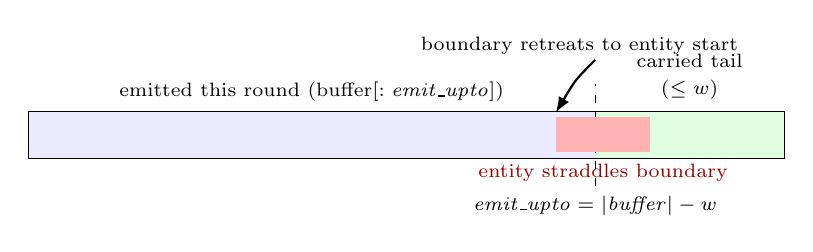
\begin{tikzpicture}[font=\small,scale=1.0]
% buffer bar
\def\y{0}
\fill[blue!8] (0,\y) rectangle (7.2,0.6);
\fill[green!12] (7.2,\y) rectangle (9.6,0.6);
\draw (0,\y) rectangle (9.6,0.6);
\draw[dashed] (7.2,-0.35) -- (7.2,0.95);
\node[above] at (3.6,0.6) {\scriptsize emitted this round (buffer$[:\mathit{emit\_upto}]$)};
\node[above,align=center] at (8.4,0.62) {\scriptsize carried tail\\[-1pt]\scriptsize ($\le w$)};
\node[below] at (7.2,-0.35) {\scriptsize $\mathit{emit\_upto} = |\mathit{buffer}| - w$};
% straddling entity
\fill[red!30] (6.7,0.08) rectangle (7.9,0.52);
\node[below,red!60!black] at (7.3,0.05) {\scriptsize entity straddles boundary};
% retreat arrow
\draw[-{Latex[length=2mm]},thick] (7.2,1.25) .. controls (6.95,1.0) .. (6.7,0.58);
\node[above] at (7.0,1.2) {\scriptsize boundary retreats to entity start};
\end{tikzpicture}
\caption{Bounded-overlap emission. Only text at least $w$ from the buffer end is
emitted; an entity straddling the emit boundary pulls the boundary back to its
start and is carried whole into the next window. Any span of length $\le w$ is
therefore seen intact at least once, regardless of where chunks fall.}
\label{fig:overlap}
\end{figure}

\begin{algorithm}[t]
\caption{Bounded-overlap streaming (sequential engine $\Sw$).}
\label{alg:stream}
\begin{algorithmic}[1]
\small
\Require chunk iterator; detector $\mathrm{detect}(\cdot)$; overlap $w$
\State $\mathit{prefix} \gets \text{``''}$; \quad $\mathit{buffer} \gets \text{``''}$
\For{each $\mathit{chunk}$}
  \State $\mathit{buffer} \gets \mathit{buffer} \mathbin{\|} \mathit{chunk}$
  \If{$|\mathit{buffer}| \le w$} \textbf{continue} \EndIf
  \State $\mathit{emit\_upto} \gets |\mathit{buffer}| - w$
  \State $D \gets \mathrm{detect}(\mathit{prefix} \mathbin{\|} \mathit{buffer})$,
         offsets shifted by $-|\mathit{prefix}|$; drop spans with start $<0$
  \State \textbf{retreat:} \textbf{while} some $d\in D$ has
         $d.\mathit{start} < \mathit{emit\_upto} < d.\mathit{end}$:
         $\mathit{emit\_upto} \gets \min d.\mathit{start}$
  \If{$\mathit{emit\_upto} \le 0$} \textbf{continue} \EndIf
  \State emit $(\mathit{buffer}[{:}\mathit{emit\_upto}],\;
         \{d \in D : d.\mathit{end} \le \mathit{emit\_upto}\})$
  \State $\mathit{prefix} \gets (\mathit{prefix} \mathbin{\|}
         \mathit{buffer}[{:}\mathit{emit\_upto}])[-w{:}]$
  \State $\mathit{buffer} \gets \mathit{buffer}[\mathit{emit\_upto}{:}]$
\EndFor
\State emit the final $(\mathit{buffer}, \mathrm{detect}(\mathit{prefix}
       \mathbin{\|} \mathit{buffer}))$ if non-empty
\end{algorithmic}
\end{algorithm}

\paragraph{Anchor prefilter.}
Each Tier-1 pattern declares literal \emph{anchors} every match must contain
(\texttt{AKIA}, \texttt{eyJ}, \texttt{@}, \texttt{://}, a digit, \ldots). A cheap
substring scan per window skips any regex whose anchor is absent, so
secret-sparse text runs markedly faster (about $25\times$ on such text, measured)
with \emph{provably identical} output---a differential test compares prefiltered
and unfiltered detection over fuzzed input. Prefiltering is an optimisation only;
it never changes the detection set.

\paragraph{Parallel execution (G3).}
To use multiple cores on a single file, the engine splits $\T$ into $k$
character-aligned byte ranges (respecting \texttt{\char`\\r\char`\\n} pairs and
self-synchronising encodings). Each worker redacts its range with $\Sw$ extended
by $w$ characters of \emph{scanned pad} and a further $w$ of \emph{context-only
prefix} on each interior side, so every seam-crossing span is seen whole and with
real left context. A span crossing a seam is owned by the \emph{left} worker; both
neighbours independently recompute the seam from the same bytes. An orchestrator
compares each neighbour pair's seam reports and, on any disagreement, discards the
partial outputs and redacts the whole file sequentially. This ``seam valve'' is
what makes the parallel path safe: disagreement is only possible when a span longer
than $w$ sits exactly on a seam, and the valve converts that into a transparent
fallback rather than silent character loss or duplication.

% ===========================================================================
\section{Formal Model and Equivalence Guarantees}
\label{sec:formal}

We model the whole-document pipeline as a function and prove the streaming and
parallel engines equal it under two locality assumptions whose constants are
audited from the implementation. The guarantees hold \emph{only} for pipelines
that satisfy this bounded-window, chunk-independent contract.

\subsection{Objects}
A \emph{detection} is a tuple $(i,j,\tau,c)$ with $0\le i<j\le|\T|$, type $\tau$,
and confidence $c\in[0,1]$. A \emph{detector} $D:\texttt{str}\to
\text{list of detections}$ returns spans as offsets into the string it is given.
The \emph{reference pipeline} $\Pipe:\texttt{str}\to\text{set of detections}$
runs every configured tier on the whole $\T$, applies contextual scoring over a
bounded left window, drops detections below a threshold $\theta$
(\texttt{min\_confidence}), and resolves overlaps into a sorted, pairwise-disjoint
set. Redaction is a pure rewrite of $\T$ given $\Pipe(\T)$, so equality of
detection sets implies byte-identical output; we therefore state the theorems over
detection sets. The streaming engine $\Sw$ (Algorithm~\ref{alg:stream}) and the
parallel engine $\Pwk$ ($k$ workers) are as defined in Section~\ref{sec:algo};
$\Sw(\T)$ and $\Pwk(\T)$ denote their emitted detections with offsets mapped back
to absolute positions.

\subsection{Assumptions and audited constants}
\begin{description}
\item[A1 (bounded span length).] Every detection in $\Pipe(\T)$ has length
$j-i \le \Lmax$.
\item[A2 (bounded context locality).] For every detection $s=(i,j,\cdot,\cdot)$,
whether $s\in\Pipe(\T)$ and its final confidence depend only on the substring
$\T[\,i-\Cleft : j+\Cright\,]$.
\end{description}
A2 says the pipeline never needs more than $\Cleft$ characters left or $\Cright$
right of a span to decide it; A1 says no span exceeds $\Lmax$. The constants are
derived \emph{mechanically} as the maximum over the default pipeline of the
bounded-window requirements each tier declares (Table~\ref{tab:constants}); a
regression test recomputes them from the shipped detectors and fails if any tier
reads wider context, so the audited values cannot silently drift from the code.
The governing left context is the $96$-character cue$\rightarrow$value window of
the default-on label-anchored identifier cascade; the base tiers read less (the
contextual scorer reads $48$). The widest declared right context is that
cascade's $8$-character bound (the base tiers' widest is a two-character negative
lookahead; every validator reads only the matched text). Two historically long
patterns (private-key PEM bodies and high-entropy runs) are explicitly bounded to
the default overlap: the private-key span is capped at exactly $8192$ characters
by bounding its key-type fields and body, and the entropy candidates are capped
at $8192$ with longer runs emitted as consecutive capped spans (covering the
whole run with no gap). Hence $\max(\Cleft,\Cright)=96 \le \Lmax = 8192 = w =
\texttt{DEFAULT\_OVERLAP}$, so the premise $w\ge\max(\Lmax,\Cleft,\Cright)$ holds
\emph{unconditionally at the default configuration} for the built-in tiers.

\begin{table}[t]
\centering
\caption{Locality constants audited from the implementation (characters). These
define the detector contract under which Theorems~\ref{thm:stream}--\ref{thm:mem}
hold; they are read from the code, not assumed.}
\label{tab:constants}
\begin{tabular}{@{}lcl@{}}
\toprule
Constant & Value & Source in implementation \\
\midrule
$\Cleft$ (left context) & $96$ & label-anchored cascade cue$\rightarrow$value window (base tiers: $48$) \\
$\Cright$ (right context) & $8$ & label-anchored cascade bound (base tiers: $2$) \\
$\Lmax$ (max span) & $8192$ & private-key bound; entropy candidate cap \\
$w$ (default overlap) & $8192$ & engine \texttt{DEFAULT\_OVERLAP} \\
$\mathit{chunk\_size}$ & $65536$ & default read size (64\,KiB) \\
\bottomrule
\end{tabular}
\end{table}

\subsection{Theorems}

\begin{theorem}[Streaming equivalence]
\label{thm:stream}
For any pipeline $\Pipe$ satisfying A1 and A2, if $w \ge
\max(\Lmax,\Cleft,\Cright)$ then $\Sw(\T)=\Pipe(\T)$ for every $\T$ and every
chunking of $\T$.
\end{theorem}

\begin{proof}[Proof sketch]
\emph{(a) Completeness.} The engine emits only text at least $w$ from the buffer
end and retreats the emit boundary to the start of any straddling detection; the
retreated tail, of length at most $\Lmax\le w$, is carried into the next window.
Hence any span cut by a chunk boundary is reassembled and presented whole to
$\mathrm{detect}$ in the next window.
\emph{(b) Soundness.} Each window is $\mathrm{detect}(\mathit{prefix}\,\|\,
\mathit{buffer})$ where $\mathit{prefix}$ is the last $w\ge\Cleft$ emitted
characters, so every span's left context is real text. A span is emitted only
when it ends at least $w\ge\Cright$ characters before the buffer's live end, so
its right context is real text too. By A2 the window verdict and confidence equal
the whole-document values; detections falling inside $\mathit{prefix}$ are
dropped.
\emph{(c) Exactly once.} A span is emitted in the unique segment whose
$\mathit{emit\_upto}$ first exceeds its end, and the carried region is disjoint
from the emitted region.
Together (a)--(c) give $\Sw(\T)=\Pipe(\T)$; byte-identity of output follows
because the rewrite is a pure function of $(\T,\Pipe(\T))$. \qed
\end{proof}

\begin{theorem}[Parallel byte-identity, with safe fallback]
\label{thm:par}
Under A1 with $w\ge\Lmax$, $\Pwk(\T)=\Sw(\T)$ byte-for-byte. When A1 is violated
at a seam, the seam valve detects the disagreement and $\Pwk$ falls back to
$\Sw$. Thus $\Pwk(\T)=\Sw(\T)$ \emph{unconditionally}, and the parallel path never
silently diverges from the sequential one.
\end{theorem}

\begin{proof}[Proof sketch]
Character-aligned ranges decoded with the same incremental decoder reproduce the
sequential substring exactly. Each worker prepends $w$ characters of scanned pad
and $w$ of context-only prefix, so with $w\ge\Lmax$ (A1) and $w\ge\Cleft$ (A2)
every seam-crossing span is seen whole with real left context---the
Theorem~\ref{thm:stream} conditions applied per range. A seam-crossing span is
owned by the left worker; both neighbours recompute the seam from identical
bytes. The orchestrator compares seam reports and falls back to $\Sw$ on any
mismatch. A mismatch is possible only when a span longer than $w$ sits on a seam,
i.e.\ exactly when A1 fails; so the valve turns every A1 violation into a
transparent fallback. \qed
\end{proof}

\begin{theorem}[Constant-memory bound]
\label{thm:mem}
Peak working memory of $\Sw$ is at most $\mathit{chunk\_size}+w+\Lmax$,
independent of $|\T|$; $\Pwk$ uses at most $k$ times that.
\end{theorem}

\begin{proof}[Proof sketch]
After each emit the engine retains only the carried region (at most $w$ plus one
straddling span of length $\le\Lmax$); the next iteration adds at most one
$\mathit{chunk\_size}$ chunk before emitting again. The buffer therefore never
exceeds $\mathit{chunk\_size}+w+\Lmax$ regardless of $|\T|$. Each worker runs one
$\Sw$ plus a $2w$ holdback, so total memory scales with $k$, never with
$|\T|$. \qed
\end{proof}

\subsection{Where the guarantee stops}
\label{sec:limits}
The assumptions fail in exactly these cases, all detectable or documented.
(i)~A span longer than $w$: no built-in tier produces one at the default overlap,
but a user may lower $w$, add a custom detector with an unbounded span, or supply
a single high-entropy run longer than $w$; in sequential mode such a span may be
split, and in parallel mode the seam valve falls back. (ii)~A detector needing
unbounded right context: A2 fixes a small finite $\Cright$, so any future tier
that conditions on a whole document---most notably a large-language-model
tier---breaks A2, and
\emph{neither theorem applies to it}. This is the principled reason the bounded,
offline tiers are the ones that carry the equivalence guarantee. We note that the
optional NER and ONNX tiers declare a bounded ($256$-character) context window but
are statistical models whose effective context may exceed it near a chunk
boundary; their accuracy there is a documented limitation the overlap mitigates
but does not eliminate, and we do not extend the byte-exact equivalence claim to
them. (iii)~Non-splittable encodings fall back to the sequential path by
construction, to which Theorem~\ref{thm:stream} still applies.

% ===========================================================================
\section{Semantic Detection Ensemble and Policy Calibration}
\label{sec:semantic}

\paragraph{Calibrated confidences (G6).}
The built-in tier confidences are hand-set constants that order detections
sensibly but are not probabilities. To remove the ``you just picked $0.5$''
objection, a dependency-free logistic \emph{calibrator} maps each detection to a
probability of being a true positive from detection-\emph{local} features only:
the raw confidence, a one-hot of the producing tier, whether context boosted or
suppressed it, and whether its type is structured (checksum/grammar-backed) or
free-form. Crucially every feature is a function of the detection alone, so
applying the calibrator changes the reference pipeline $\Pipe$ but
\emph{preserves} the equivalence of $\Sw$/$\Pwk$ to $\Pipe$
(Theorems~\ref{thm:stream}--\ref{thm:par}). The accompanying harness trains the
calibrator on a labelled corpus and reports Brier score and expected calibration
error before versus after, plus a per-tier ablation (the marginal micro-F1 of the
entropy and NER tiers). The calibrator is the mechanism; the labelled corpus and
the resulting calibration numbers are supplied by the user under their own data
licences and are \emph{not} bundled in the repository, so we report the method
rather than a specific trained model's scores.

\paragraph{Two operating points: strict and high\_recall.}
The ensemble exposes a single threshold $\theta$ (\texttt{min\_confidence}) that,
together with the contextual tier, defines two named policies:
\begin{description}
\item[\textsc{strict} (default, $\theta=0.5$).] Precision-favouring. The
contextual tier \emph{subtracts} confidence from values adjacent to placeholder
markers (``example'', ``test'', ``sample'', \ldots), so documentation snippets
and fixture data are left untouched. The side effect is that a file
\emph{saturated} with marker words under-detects---working as designed.
\item[\textsc{high\_recall} ($\theta\approx0.35$, NER enabled).] Recall-favouring.
Lowering the threshold recovers most values the placeholder suppression demotes,
at some precision cost, and enabling the NER tier adds free-text names; intended
for data known to be noisy rather than for trusted prose.
\end{description}
These are operating points on one precision/recall curve, selected per run, not
separate detectors.

\paragraph{Named-entity tiers as an integration interface.}
Free-text PERSON/ORG/LOC recognition is delegated to an optional spaCy tier or a
local ONNX token-classification tier. The ONNX tier is a \emph{model-integration
interface}: it provides a pure, unit-tested BIO/IOB2 decoder and pluggable
tokeniser/backend seams, and runs any supplied on-device model under the offline
guard with no data egress. The repository contains no benchmark of a concrete
ONNX (or GLiNER-class) model, so we present ONNX strictly as an integration path
and report \emph{no} accuracy numbers for it; doing otherwise would misrepresent
a mock as a measured result.

\paragraph{The trade-off, stated honestly.}
Perfect recall and perfect precision together are unattainable for free-text PII
by any tool: a bank-account number is indistinguishable from any other run of
digits, and ``April'' is both a name and a month. SafeStream is tuned to favour
precision on structured PII and credentials, with names and format-less
identifiers handled by the opt-in levers above. We therefore report results as a
precision/recall and benign-false-positive trade-off (Section~\ref{sec:eval}),
and explicitly do \emph{not} claim that semantic/free-text recall is solved.

% ===========================================================================
\section{Experimental Evaluation}
\label{sec:eval}

\paragraph{Scope and honesty of the corpora.}
The corpora used for the accuracy numbers below are \emph{synthetic and
self-generated}: gold positives are emitted in the canonical formats the
detector targets. A near-perfect score on them therefore measures \emph{format
coverage and false-positive resistance}, not real-world recall. They are a
regression fixture, not an accuracy claim. The repository ships an evaluation
harness (\texttt{evaluate.py}) with bootstrap confidence intervals, a paired
significance test, CoNLL-2003/Presidio-dataset loaders, and baseline adapters
(regex, Presidio with NER, scrubadub, gitleaks) for running on independent
labelled corpora (Presidio research dataset, CoNLL-2003, the n2c2 clinical
de-identification set~\cite{conll2003,n2c2}); those corpora carry their own
licences and are supplied by the user, so the real-world accuracy study is
enabled but not bundled. All numbers reported here are SafeStream's own measured
values from the repository's recorded results; competitor rows are clearly
labelled as to provenance.

\paragraph{Environment.}
Recorded results were produced on CPython 3.11.15, Linux x86-64, an Intel Xeon at
2.10\,GHz (4 cores, a shared/throttled vCPU), 16\,GB RAM, package version 0.2.0.
Throughput is environment-specific on this throttled vCPU and should be read as
\emph{relative}, not a hardware ceiling.

\subsection{Format coverage and false-positive resistance}
Table~\ref{tab:accuracy} reports the deterministic tier on two self-generated
corpora. Matching is type-aware with at least $50\%$ span overlap; the types are
email, phone, credit card, SSN, and IPv4---the set the deterministic tier and a
pattern baseline both cover. The clean-corpus $\mathrm{F1}=1.000$ is a regression
fixture and is close to circular. The \emph{informative} number is the
adversarial precision: on $5.2$\,MB dense with hard negatives (Luhn-failing
16-digit numbers, 5-octet version strings, invalid-area SSNs, ISO timestamps,
UUIDs, git hashes), the validators reject almost all distractors, leaving only
$45$ benign false positives across $70{,}169$ gold spans ($\mathrm{P}=0.999$).
This is the benign-false-positive side of the trade-off in
Section~\ref{sec:semantic}, measured.

\begin{table}[t]
\centering
\caption{Measured accuracy and throughput on self-generated corpora
(type-aware matching, $\ge 50\%$ overlap; types: email, phone, credit\_card, ssn,
ipv4). These measure format coverage and false-positive resistance, \emph{not}
real-world recall.}
\label{tab:accuracy}
\setlength{\tabcolsep}{5pt}
\begin{tabular}{@{}lrrrrrrrr@{}}
\toprule
Corpus & Size & Gold & P & R$^\ast$ & F1 & FP & FN & MB/s \\
\midrule
Clean / canonical     & 10.5\,MB & 60{,}253 & 1.000 & 1.000 & 1.000 & 0  & 0 & 3.50 \\
Adversarial (hard neg.) & 5.2\,MB  & 70{,}169 & 0.999 & 1.000 & 1.000 & 45 & 0 & 2.06 \\
\bottomrule
\end{tabular}
\\[2pt]
{\footnotesize $^\ast$ Recall is against self-generated positives and is
\emph{not} a real-world recall figure; the non-circular result is the precision
under distractors.}
\end{table}

\subsection{Constant memory}
Table~\ref{tab:memory} reports peak Python-heap allocations (via
\texttt{tracemalloc}) as input grows. A $4\times$ increase in input produces
\emph{zero} increase in peak allocation---the empirical signature of
Theorem~\ref{thm:mem}. A repository test corroborates the property three orders
of magnitude larger: a $\sim\!1$\,GB generated file redacts with peak allocations
under a $16$\,MB cap.

\begin{table}[t]
\centering
\caption{Measured constant-memory scaling (peak \texttt{tracemalloc}
allocations; $w=8$\,KiB, $\mathit{chunk\_size}=64$\,KiB, single worker).}
\label{tab:memory}
\begin{tabular}{@{}lrr@{}}
\toprule
Input size & Peak memory & Ratio to smallest \\
\midrule
8\,MB  & 2.75\,MB & $1.00\times$ \\
32\,MB & 2.75\,MB & $1.00\times$ \\
1\,GB (repository test) & $<16$\,MB (asserted) & --- \\
\bottomrule
\end{tabular}
\end{table}

\subsection{Parallel byte-identity and scanning speed}
Parallel byte-identity (Theorem~\ref{thm:par}) is enforced continuously: the
test suite and the speedup harness assert that splitting a file across workers
produces output byte-identical to the sequential pass at every worker count, or
falls back via the seam valve. A prior run recorded about $3.7\times$ speedup on
4 cores. The anchor prefilter yields about $25\times$ on secret-sparse text with
provably identical output. We are candid that raw single-core throughput
($2$--$3.5$\,MB/s on this throttled vCPU) is a known limitation, not a strength:
compiled scanners are expected to be far faster (not measured here). A drop-in re2/Vectorscan
backend was prototyped and measured but \emph{not adopted}, because re2's
ASCII-only word boundaries change detection output on Unicode text and it cannot
compile the lookaround the throughput-dominating PII patterns use; the value here
is constant memory, dual PII+secret coverage, and the equivalence guarantee,
not speed.

\subsection{Capability comparison with existing systems}
Table~\ref{tab:capability} summarises a \emph{documentation-based} capability
comparison (abridged) against widely used systems. Only SafeStream's cells are
\emph{measured} in the repository; every competitor cell reflects
\emph{documented} capability from public sources and is labelled as such. A blank
or ``?'' means \emph{not documented}, not ``no''. Separately, Table~\ref{tab:presidio} gives a head-to-head against Presidio
produced by one harness (\texttt{benchmarks/presidio\_compare.py}, one run on a
4-vCPU shared container) and grouped into \emph{like-for-like tiers}: in the pattern
tier SafeStream's rule-based tiers are compared with Presidio's own pattern
recognizers run directly, with no NLP engine; in the NER tier both run on the same
spaCy \texttt{en\_core\_web\_sm} model. Comparing SafeStream's native core with
Presidio's \emph{full} default engine (spaCy \texttt{en\_core\_web\_lg}) yields
$281$--$543\times$, but that contrasts regex with regex-plus-NLP and we do not claim
it. Like-for-like the speed advantage is $15$--$147\times$ in the pattern tier and
about $2\times$ in the NER tier, where SafeStream also uses about $2.5\times$ more
memory than Presidio and Presidio's entity recall is higher ($0.659$ versus $0.520$).
The synthetic-log corpus is generated by this work in the formats SafeStream
targets, so its near-perfect recall measures format coverage and false-positive
resistance, not real-world recall; on real prose (RedactionBench) neither tool
exceeds $0.54$ character recall. Hyperscan/re2, gitleaks and the ONNX tier were not
measured. Presidio ships no credential recognizers ($0/9$ versus $9/9$ on a
credential corpus), a \emph{capability} difference rather than a tuned accuracy
comparison. Presidio's spaCy/transformer NER tier is a separate, model-dependent
path that out-recalls a regex core on free-text names.

\begin{table}[t]
\centering
\caption{Like-for-like comparison with Presidio (one run; P/R are character
precision/recall; speed is SafeStream $\div$ Presidio throughput). Memory is
tool RSS, SafeStream/Presidio.}
\label{tab:presidio}
\begin{tabular}{@{}llrrr@{}}
\toprule
Tier & Corpus & SafeStream P/R & Presidio P/R & Speed \\
\midrule
Pattern, native & logs & $0.999/1.000$ & $0.741/0.865$ & $147\times$ \\
Pattern, native & RedactionBench & $0.754/0.412$ & $0.422/0.292$ & $42\times$ \\
Pattern, Python & logs / RedactionBench & (same as native) & (same) & $33\times$ / $15\times$ \\
NER, \texttt{sm} both & RedactionBench & $0.547/0.540$ & $0.364/0.455$ & $2.0\times$ \\
\bottomrule
\end{tabular}
\end{table}

\begin{table}[t]
\centering
\caption{Abridged capability comparison (documented; SafeStream measured where
noted). $\bullet$ documented yes, $\circ$ no/limited, $\blacktriangle$
optional/add-on, ? unknown. Full matrix against ten systems is in the
repository.}
\label{tab:capability}
\setlength{\tabcolsep}{3.5pt}
\begin{tabular}{@{}lccccc@{}}
\toprule
Capability & SafeStream & Presidio & Philter & \makecell{gitleaks-\\class} & \makecell{Cloud\\DLP} \\
\midrule
Runs fully offline / local      & $\bullet$ & $\bullet$ & $\bullet$ & $\bullet$ & $\circ$ \\
PII detection                   & $\bullet$ & $\bullet$ & $\bullet$ & $\blacktriangle$ & $\bullet$ \\
Credential / secret detection   & $\bullet$ & $\circ$ & $\circ$ & $\bullet$ & $\blacktriangle$ \\
High-entropy secret detection   & $\bullet$ & $\circ$ & $\circ$ & $\bullet$ & $\circ$ \\
ML / NER detection              & $\blacktriangle$ & $\bullet$ & $\bullet$ & $\circ$ & $\bullet$ \\
Streaming / large-file input    & $\bullet$ & $\circ$ & ? & $\bullet$ & $\bullet$ \\
Bounded / constant memory       & $\bullet$ (meas.) & $\circ$ & ? & ? & N/A \\
No data leaves the machine      & $\bullet$ & $\bullet$ & $\bullet$ & $\bullet$ & $\circ$ \\
\bottomrule
\end{tabular}
\end{table}

% ===========================================================================
\section{Discussion and Threats to Validity}
\label{sec:discussion}

\paragraph{Construct validity.}
The headline accuracy corpora are synthetic and self-generated; their
near-perfect recall is by construction and is \emph{not} evidence of real-world
recall. We mitigate this by (i) reporting precision under adversarial distractors
as the informative number, (ii) framing the clean corpus explicitly as a
regression fixture, and (iii) shipping a harness that runs the same scoring on
independent labelled corpora with confidence intervals and significance tests.
The honest state of a regex-first detector is high recall on structured PII and
credentials and substantially lower recall on free-form names/addresses without
the NER tier.

\paragraph{Internal validity.}
The equivalence theorems depend on assumptions A1/A2 and apply only to detectors
satisfying the bounded-window, chunk-independent contract. We audited the
constants from the code rather than assuming them, and the built-in tiers satisfy
the contract at the default overlap; a custom detector or a lowered overlap can
violate A1, which in parallel mode is caught by the seam valve and in sequential
mode is surfaced by a runtime warning. Statistical NER tiers are outside the
byte-exact claim by design.

\paragraph{External validity.}
Throughput was measured on a single throttled vCPU and is relative; the
capability comparison against other systems is documentation-based except for the
single-run Presidio head-to-head (Table~\ref{tab:presidio}; one run, no repeats, so
ratios near $2\times$ are within scheduling noise), and cloud/commercial systems,
Hyperscan/re2, gitleaks and the ONNX tier were not benchmarked (they
require credentials, cost approval, and terms permitting publication). We
therefore label measured, prior-measured, and documented claims distinctly
throughout.

\paragraph{Security caveats.}
The in-process network guard is best-effort defence-in-depth, not a hard
boundary; a kernel-enforced mode and container isolation are the stronger
options. Deterministic keyed pseudonymisation preserves referential integrity but
leaks value equality and is invertible by a key holder over low-cardinality
domains; it is not anonymisation. These are stated so that the guarantees are not
over-read.

% ===========================================================================
\section{Conclusion}
\label{sec:conclusion}

SafeStream-Redactor shows that a redactor can be simultaneously
\emph{constant-memory}, \emph{parallel}, and \emph{provably output-equivalent} to
a whole-document pass---under assumptions that are stated precisely, audited from
the implementation, and bounded by a named, safely-handled failure mode. It
covers PII and credentials in a single local-first pass, and exposes a calibrated
precision/recall knob with \textsc{strict} and \textsc{high\_recall} operating
points. We deliberately do not claim to solve free-text recall, and we separate
measured from documented results throughout. The contribution is the guarantee
the engineering admits: a bounded-memory parallel redactor whose output matches
an idealised whole-document pass, with the one place the guarantee stops made
explicit and safe. Future work is the independent-corpus accuracy study the
bundled harness already supports, and principled integration of statistical and
model-based tiers that, by design, fall outside the byte-exact equivalence claim.

% ===========================================================================
% References --- LNCS numbered style, embedded for a self-contained source.
\begin{thebibliography}{99}

\bibitem{gdpr}
European Parliament and Council of the European Union:
Regulation (EU) 2016/679 (General Data Protection Regulation).
Official Journal of the European Union L119, 1--88 (2016)

\bibitem{presidio}
Microsoft: Presidio --- Data Protection and De-identification SDK.
\url{https://github.com/microsoft/presidio} (last accessed 2026)

\bibitem{philter}
Norgeot, B., Muenzen, K., Peterson, T.A., Fan, X., Glicksberg, B.S., Schenk, G.,
Rutenberg, E., Oskotsky, B., Sirota, M., Yazdany, J., Schmajuk, G., Ludwig, D.,
Goldstein, T., Butte, A.J.:
Protected Health Information Filter (Philter): Accurately and Securely
De-identifying Free-text Clinical Notes. npj Digital Medicine 3, 57 (2020)

\bibitem{n2c2}
Stubbs, A., Kotfila, C., Uzuner, \"{O}.:
Automated Systems for the De-identification of Longitudinal Clinical Narratives:
Overview of 2014 i2b2/UTHealth Shared Task Track 1.
Journal of Biomedical Informatics 58, S11--S19 (2015)

\bibitem{conll2003}
Tjong Kim Sang, E.F., De Meulder, F.:
Introduction to the CoNLL-2003 Shared Task: Language-Independent Named Entity
Recognition. In: Proc.\ CoNLL-2003, pp.\ 142--147 (2003)

\bibitem{bert}
Devlin, J., Chang, M.-W., Lee, K., Toutanova, K.:
BERT: Pre-training of Deep Bidirectional Transformers for Language Understanding.
In: Proc.\ NAACL-HLT, pp.\ 4171--4186 (2019)

\bibitem{gliner}
Zaratiana, U., Tomeh, N., Holat, P., Charnois, T.:
GLiNER: Generalist Model for Named Entity Recognition using Bidirectional
Transformer. In: Proc.\ NAACL-HLT, pp.\ 5364--5376 (2024)

\bibitem{nersurvey}
Li, J., Sun, A., Han, J., Li, C.:
A Survey on Deep Learning for Named Entity Recognition.
IEEE Transactions on Knowledge and Data Engineering 34(1), 50--70 (2022)

\bibitem{howbadgit}
Meli, M., McNiece, M.R., Reaves, B.:
How Bad Can It Git? Characterizing Secret Leakage in Public GitHub Repositories.
In: Proc.\ Network and Distributed System Security Symposium (NDSS) (2019)

\bibitem{secretbench}
Basak, S.K., Neil, L., Reaves, B., Williams, L.:
SecretBench: A Dataset of Software Secrets.
In: Proc.\ IEEE/ACM 20th International Conference on Mining Software Repositories
(MSR), pp.\ 347--351 (2023)

\bibitem{gitleaks}
Rice, Z.: gitleaks --- Find secrets and detect hardcoded credentials.
\url{https://github.com/gitleaks/gitleaks} (last accessed 2026)

\bibitem{shannon}
Shannon, C.E.:
A Mathematical Theory of Communication.
The Bell System Technical Journal 27(3), 379--423 (1948)

\bibitem{muthukrishnan}
Muthukrishnan, S.:
Data Streams: Algorithms and Applications.
Foundations and Trends in Theoretical Computer Science 1(2), 117--236 (2005)

\bibitem{thompson}
Thompson, K.:
Programming Techniques: Regular Expression Search Algorithm.
Communications of the ACM 11(6), 419--422 (1968)

\bibitem{re2}
Cox, R.:
Regular Expression Matching Can Be Simple And Fast (but is slow in Java, Perl,
PHP, Python, Ruby, \ldots). \url{https://swtch.com/~rsc/regexp/regexp1.html}
(2007, last accessed 2026)

\bibitem{hmac}
Krawczyk, H., Bellare, M., Canetti, R.:
HMAC: Keyed-Hashing for Message Authentication. RFC 2104, IETF (1997)

\bibitem{kanonymity}
Sweeney, L.:
k-anonymity: A Model for Protecting Privacy.
International Journal of Uncertainty, Fuzziness and Knowledge-Based Systems
10(5), 557--570 (2002)

\bibitem{luhn}
Luhn, H.P.: Computer for Verifying Numbers. U.S. Patent 2,950,048 (1960)

\end{thebibliography}

\end{document}
